\section{The Electrocardiograph}

The electrocardiograph, or ECG, was developed by Einthoven and colleagues at the
turn of the 20th century.
The Einthoven ECG used the string galvanometer, developed by Einthoven himself, to
record the potential differences between three sets of electrodes, or leads.
These electrodes were placed on each arm and on the left leg.
These three electrodes form the basis of many ECGs recorded to this day.
The string galvanometer was highly sensitive electrical recording device for its
time.
For the development of the ECG and the string galvanometer, Einthoven was awarded
the Nobel prize in 1924~\cite{Kligfield2002,Levick1991}.

Since Einthoven's day, the ECG has been continually refined.
This refinement has included both improvements in the way that individual leads
are measured, and new leads that are recorded.
In addition, there have been a number of specialised lead sets developed for
particular purposes, such as exercise recording and 24 hour measurement.
Research into new lead sets, to better understand the functioning of the heart,
continues to this
day~\cite{Jahrsdoerfer2005,Sobieszczanska2007,Grube2007,Finlay2007}.

\subsection{Lead Theory}
\label{sec:intro:ecg:lead_theory}

In Einthoven's original conception of the heart and the electrical field it
produced, he proposed the `Einthoven Triangle'.
The Einthoven triangle is an equilateral triangle.
At its corners sit the three electrodes and the sides of the triangles are the
leads themselves.
At the centroid of the triangle sits the heart, which is represented by a
single, stationary, time varying dipole.
The potentials measured at the three electrodes are the potentials assuming the
system is two dimensional, homogeneous and infinite in extent.
This is not entirely incorrect.

Modern lead theory was developed in the 1950s.
In a series of three papers McFee and
Johnston~\cite{McFee1953,McFee1954a,McFee1954b}\ set out their concept of the
`lead field' which is still considered applicable today.
This theory, which was a further generalisation of work by Burger and van
Milaan~\cite{Burger1946}, allows for a heart which consisted of distributed dipole sources
sitting in a three dimensional, finite and inhomogeneous medium.

First, it is useful to define what a lead is.
A lead is defined as a pair of terminals, each connected to any number of electrodes
on the body, either directly or through any number of resistors or amplifiers.
One of the terminals is designated (arbitrarily) as the `positive' terminal.
The terminals are connected such that a positive measurement is taken if
the `positive' terminal has a higher potential than the `negative' one.

The lead field theory is based on the fundamental principles of linear volume
conductors set out by Helmholtz in the middle of the nineteenth century.
These principles only hold if the body can be treated as a linear volume
conductor.
This is a good approximation~\cite{Geddes1967}.

The first principle, that of superposition, states that the electric field
resulting from several sources in the medium is equal to the sum of the fields
which would be produced by each source considered alone.
The second principle, that of reciprocity, concerns current flow in the
medium.
It states that the current flow between two electrodes evoked by a field source in the
medium is the same as the current flow through the source evoked by placing a
potential difference across the two electrodes equal to the potential difference
that would have been created by the field source.
That is to say that the current flow is independent of the direction of
energisation, from within or outside the medium.

\begin{figure}
\begin{center}

\includegraphics{figures/intro/lead_field}
\end{center}
\caption[Diagram of the Reciprocity Principle and the Lead Field]{
\label{fig:intro:ecg:lead_field}
Diagram of the Reciprocity Principle and the Lead Field.
(a) Inducing a current in the lead $l$, between the terminals of the
galvanometer causes an electric field which causes a current $i$ to flow through
the small element (square) in the heart.
(b) An electric field, $\vec{e}$, generated by the small element causes a current
I to flow in $l$ causing the galvanometer to read the potential difference $E'$.
If $E'$ equals $E$ then $I$ equals $i$.
(c) The lead field, $\vec{L}$, is defined from the current which flows in each
small unit of the heart when the current introduced is the unit current.

}
\end{figure}

To derive the lead field, we consider a unit current flowing in a
lead, $l$~(figure~\ref{fig:intro:ecg:lead_field}).
The resulting flow of current through the body will have a certain magnitude and
direction at every point; it is a vector field.
This vector field is called $\vec{L}$, the lead field.
If one considers a small volume in the heart region of the torso then the
presence of the lead field, $\vec{L}$, will set up an electric field in the
volume, $\vec{e}$.
The principle of reciprocity means that if instead the electrical activity of
the heart creates an electric field, $\vec{e}$, in the heart region then a unit
current will flow through the lead $l$.
The principle of superposition allows the contributions of many such small
volumes, each containing their own field, $\vec{e_1},\cdots,\vec{e_n}$, to
create a current, and thus a potential difference in $l$.


\subsection{The Twelve Lead Electrocardiogram}

The twelve lead electrocardiograph is the initial basis of almost all cardiac
diagnosis.
It started out as the three Einthoven leads.
The electrodes are located (figure~\ref{fig:intro:ecg:leads})(a)) on the left
shoulder, L, the right shoulder, R, and the feet (typically the left leg), F.
Lead I (\ref{eqn:intro:leads:i}) uses R as the negative terminal and L as the
positive terminal.
Lead II (\ref{eqn:intro:leads:ii}) is formed between R as the negative terminal
and F as the positive terminal.
Lead III (\ref{eqn:intro:leads:iii}) is formed between L as the negative terminal
and F as the positive terminal.

\begin{figure}
\begin{center}
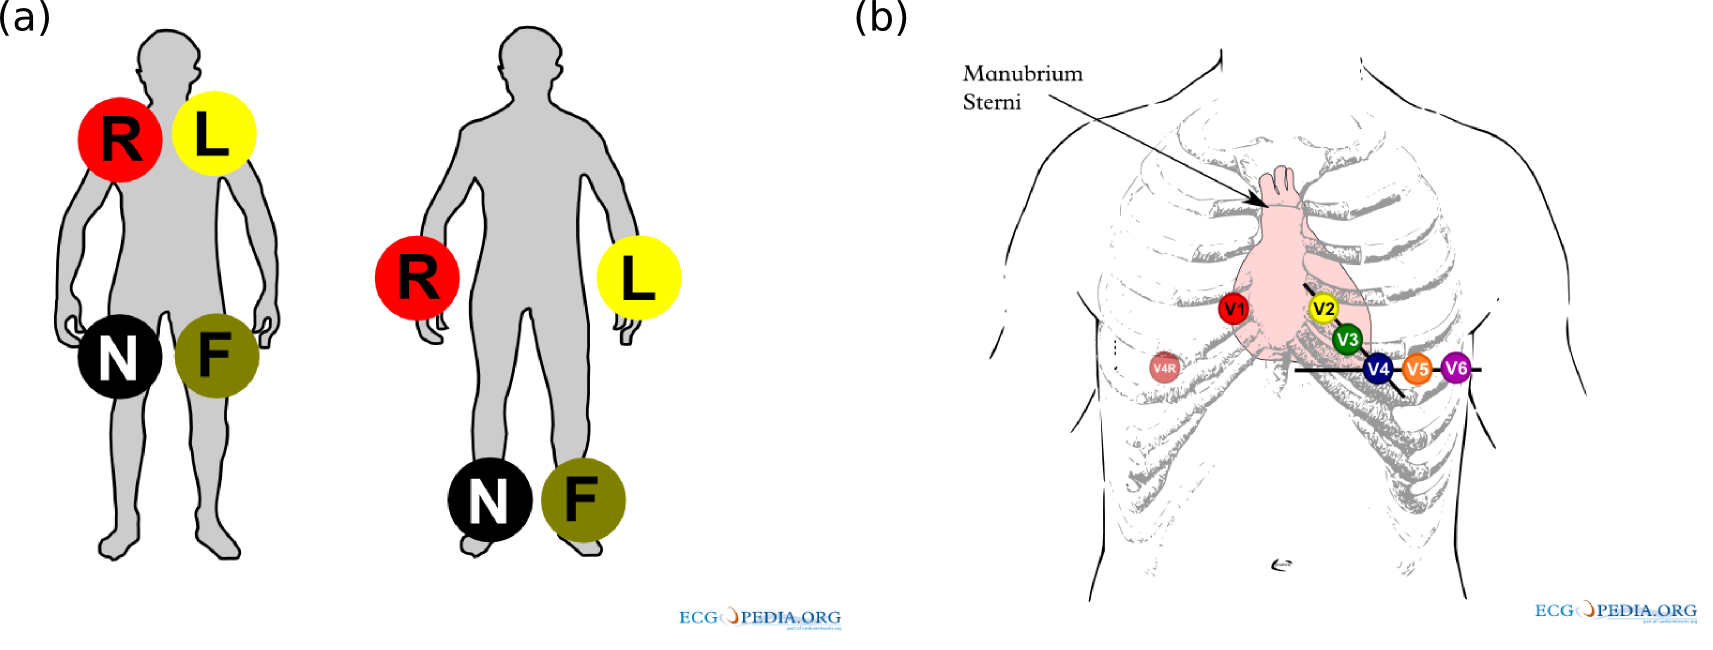
\includegraphics{figures/intro/ecg_leads}
\end{center}
\caption[Lead placements for the 12 Lead ECG]{
\label{fig:intro:ecg:leads}
Lead placements for the 12 lead ECG.
(a) Placement of the three limb leads, L, R and F, as well as the ground
electrode N.
(b) Placement of the six precordial electrodes, $\text{V}_{\text{1--6}}$.

Images are reproduced from the ECGpedia~\cite{ecgpedia}.
Both are kindly released under a Creative Commons
Attribution-Noncommercial-Share Alike 3.0 Netherlands License.
}
\end{figure}

Wilson~\cite{Wilson1934}, in the 1930s, introduced an indifferent
electrode,  constructed by averaging the potentials at the three limb
electrodes (\ref{eqn:intro:leads:wct}).
This is the Wilson's central terminal (WCT).
They introduced three new `unipolar' leads, all of which use the WCT as the
negative terminal.
For the positive terminal, VL uses the L electrode, VR the R electrode and VF
the F electrode.
Later Goldberger~\cite{Goldberger1942}\ noted that by removing the electrode used
as the positive terminal from the calculation of the central terminal for the
negative electrode, the amplitude of the lead would be 50 per cent larger than
that of the normal unipolar leads.
These leads were termed the augmented unipolar leads, denoted by the prefix of
an `a'.
The aVL (\ref{eqn:intro:leads:avl}) leads uses L for the positive terminal and
the average of R and F for the negative terminal.
The aVR (\ref{eqn:intro:leads:avr}) leads uses R for the positive terminal and
the average of L and F for the negative terminal.
The aVF (\ref{eqn:intro:leads:avf}) leads uses F for the positive terminal and
the average of R and L for the negative terminal.
The set of leads consisting of I, II, III, aVL, aVR and aVF are known as the
limb leads.
The superior limb leads are I, aVL, aVR and the inferior are II, III, aVF.

The precordial leads were introduced by Wilson~\cite{Wilson1944}\ to provide a
better view of the electrical activity of the heart from the chest.
They are all unipolar leads which use the WCT for the negative
terminal.
For the positive terminal they use one of the six precordial electrodes
(figure~\ref{fig:intro:ecg:leads})(b), the locations of which are described in
many textbooks (e.g.  \cite{Hampton2008}).
The first precordial electrode, which is the positive terminal of
$\text{V}_{\text{1}}$ (\ref{eqn:intro:leads:v1}) is located to the right of the
sternum, in the fourth intercostal--between the ribs--space.
The second precordial electrode, which is the positive terminal of
$\text{V}_{\text{2}}$ (\ref{eqn:intro:leads:v2}) is located to the left of the
sternum, in the fourth intercostal space.
The third, the positive terminal of $\text{V}_{\text{3}}$
(\ref{eqn:intro:leads:v3}) is located between the second and fourth precordial
electrodes.
The fourth ($\text{V}_{\text{4}}$, \ref{eqn:intro:leads:v4}) is located on the
left midclavicular line, in the fifth intercostal space.
The fifth ($\text{V}_{\text{5}}$, \ref{eqn:intro:leads:v5}) is located on the
left anterior axillary line, in the fifth intercostal space.
The sixth ($\text{V}_{\text{6}}$, \ref{eqn:intro:leads:v6}) is located on the
left posterior axillary line, in the fifth intercostal space.

The voltage, $V$, across each lead can be written as
\begin{subequations} \label{eqn:intro:leads}
\begin{align}
V_{I}  = &\phi_{L} - \phi_{R}\label{eqn:intro:leads:i}\\
V_{II}  = &\phi_{R} - \phi_{F}\label{eqn:intro:leads:ii} \\
V_{III}  = &\phi_{L} - \phi_{F}\label{eqn:intro:leads:iii}\\
V_{WCT}  = &\frac{\phi_{L} + \phi_{R} + \phi_{F}}{3}\label{eqn:intro:leads:wct}\\
V_{aVL} = &\phi_{L} - \left(\frac{\phi_{R} + \phi_{F}}{2}\right) \label{eqn:intro:leads:avl}\\
V_{aVR} = &\phi_{R} - \left(\frac{\phi_{L} + \phi_{F}}{2}\right)\label{eqn:intro:leads:avr} \\
V_{aVF} = & \phi_{F} - \left(\frac{\phi_{R} + \phi_{L}}{2}\right)\label{eqn:intro:leads:avf}\\
V_{1} = & \phi_1 - V_{WCT} \label{eqn:intro:leads:v1}\\
V_{2} = & \phi_2 - V_{WCT} \label{eqn:intro:leads:v2}\\
V_{3} = & \phi_3 - V_{WCT} \label{eqn:intro:leads:v3}\\
V_{4} = & \phi_4 - V_{WCT} \label{eqn:intro:leads:v4}\\
V_{5} = & \phi_5 - V_{WCT} \label{eqn:intro:leads:v5}\\
V_{6} = & \phi_6 - V_{WCT} \label{eqn:intro:leads:v6}
\end{align}
\end{subequations}
where $\phi_x$ is the potential measured at electrode $x$.

As there are only 9 electrodes in the twelve lead ECG, there are only 8
potential differences which can be uniquely determined.
These are, by convention, leads I, II and $\text{V}_{\text{1--6}}$.
The value of the other limb leads is that they provide a view of the activity of
the heart from different angles, thus what might be unclear on one lead can be
obvious on another.
This concept of lead angles creates what is known as the hexaxial reference
system (\cite{Lipman1994}, pp 94., amongst others), illustrated in
figure~\ref{fig:intro:ecg:hex}.
The angle at which each lead points is the direction of the positive terminal.
Lead I, which is nominally horizontal, is at \degr{+0}.
Under the hexaxial system, Lead II has an angle of \degr{+60}\ and lead III,
\degr{+120}.
The unipolar limb leads (both augmented and not) have angles of \degr{-30}\ for
aVL, \degr{+90}\ for aVF and \degr{-150}\ for aVR.

\begin{figure}
\begin{center}

\includegraphics{figures/intro/hexaxial}
\end{center}
\caption[Hexaxial Reference System]{
\label{fig:intro:ecg:hex}
Diagram of the hexaxial reference reference system, showing the nominal
directions of the 6 limb leads.
The positive senses of the leads are in bold, the negative are dashed.
\degr{+0}\ is horizontal and to the left, in the reference frame of the body.
}
\end{figure}

\subsection{The ECG Waves}

\begin{figure}
\begin{center}

\includegraphics{figures/intro/schematic_ecg}
\end{center}
\caption[Schematic ECG]{
\label{fig:intro:ecg:schematic}
A schematic representation of the ECG in lead II.
Shown are the P-wave, the QRS complex and the T-wave.
Also indicated are two important time periods; the PR interval and the QT
interval.
}
\end{figure}

In terms of the ECG, a `wave' is a deflection from the baseline observed in the
lead.
There are five standard waves in the ECG; P, Q, R, S and T.
The origin of the names of these waves is a matter of some
controversy~\cite{Hurst1998}, but whatever their origin, they are now enshrined
in the literature.
A schematic representation of the ECG waves is shown in
figure~\ref{fig:intro:ecg:schematic}.
Each of the waves is the result of the electrical activity in a particular part
of the heart.
Positive deflections are those which are above the baseline and negative ones
below.

The P-wave is caused by the depolarisation of the atria.
It has a relatively low amplitude because the atria are small and thin walled
compared to the ventricles, so there are not that many cells which can generate
the wave.
It tends to last from \ms{100} to \ms{120}.

The QRS complex is associated with the ventricular depolarisation.
It is a collection of up to three waves.
Any negative deflection which preceeds the R wave is the Q wave.
The R wave is the first positive deflection.
The S wave is the first negative deflection after the R wave.
A QRS complex does not need to have all three of the QRS waves present.
The QRS complex tends to have the largest magnitude in the ECG and lasts
approximately \ms{100}.

The T wave is associated with the ventricular repolarization.
It occurs some time after the QRS complex.
The $\text{T}_{\text{P}}$, caused by the atrial repolarization is not normally
visible on the ECG for a number of reasons.
It is very small in magnitude, it is also often masked either by the QRS complex
or by so called `baseline correction' algorithms which use the PR interval to
determine a `zero' for the ECG.

The axis of a wave is the direction in which it has maximum amplitude according
to the hexaxial reference system.
A normal QRS complex (\cite{Lipman1994,Katz2006}) has an axis between \degr{-30}\
and \degr{+110}.
A normal P wave axis is between \degr{+0}\ and \degr{+90}.

\subsubsection{Describing an ECG Wave}

\begin{figure}
\begin{center}

\includegraphics{figures/intro/ecg_waveforms}
\end{center}
\caption[ECG Morphology]{
\label{fig:intro:ecg:waveforms}
A schematic representation of P- and T-wave morphology.
From left to right, a positive, negative, a positive--negative biphasic and a
positive bifid wave are shown.
}
\end{figure}

The terminology used to describe ECG waves is illustrated in
figure~\ref{fig:intro:ecg:waveforms}.
Positive waves, those with a deflection above the baseline, and negative waves,
with a deflection below the baseline have already been explained.
The P- and T-waves can have more complex morphology however.
A P- or T- wave which shows both positive and negative deflections is termed
biphasic.
A positive--negative biphasic deflection is one which is first positive and then
negative.
A wave for which the converse is true is called negative--positive.
A wave which is entirely positive, or negative, but that has a notch in the
middle is described as bifid.

\subsection{The Vectorcardiogram}

Orthogonal lead systems, intended to measure the three independent components of
the heart's dipole, were first proposed in the middle of the 20th century.
Frank~\cite{Frank1956}, after experiments on physical models of the torso,
proposed his `corrected' orthogonal system.
This was corrected in the sense that the three lead vectors measured were
truly orthogonal and of equal magnitude in each of the three directions.
This included the influence of internal conductive regions and variability in
heart location.
The system uses 7 electrodes.
The three vectors chosen are X, a horizontal vector, positive to the left.
The Y vector is vertical and is positive towards the feet.
The Z vector is horizontal and positive towards the back.

\begin{figure}
\begin{center}
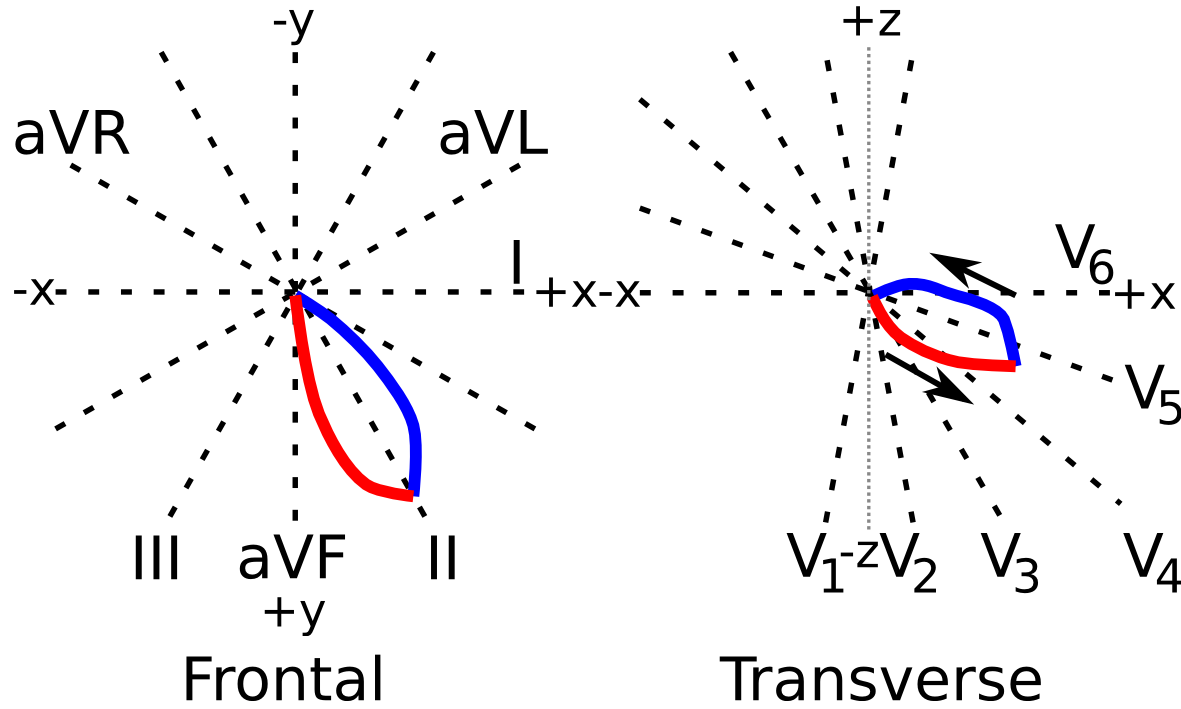
\includegraphics{figures/intro/vector_loops}
\end{center}
\caption[Schematic Vector Loops]{
\label{fig:intro:ecg:planes}
Schematic vector loops showing the relationships of the leads to the frontal and
transverse plane.
The lines of the leads are indicated in heavy-set black lines, the axes in grey
dots when they do not coincide with a lead.
The schematic loops are shown in red and blue, with arrows to indicate the
direction of inscription.
The afferent, or outgoing, limb of the loop is shown in red.
The efferent, or incoming, limb of the loop is shown in blue.
}
\end{figure}

The vectorcardiographic leads can be combined to visualize the electrical
activity of the heart in three planes.
These are the frontal plane, which combines Y and X, the transverse plane, which
combines X and Z, and the sagittal plane, which combines Y and Z.
The frontal plane is the one in which the limb leads measure, whilst the transverse plane
can be related to the precordial leads, as illustrated in
figure~\ref{fig:intro:ecg:planes}.

Dower~\cite{Dower1980}\ proposed a series of coefficients for the three Frank
leads that would convert the Frank leads into the standard 12 lead ECG.
However, the Frank leads are not recorded in common clinical practice.
To remedy this fact, Edenbrandt and Pahlm~\cite{Edenbrandt1988} (and others, for
example~\cite{Uijen1988}), proposed an `inverse dower' transformation.
The inverse dower transform is a set of $8\times3$ coefficients
(table~\ref{tbl:intro:ecg:inverse_dower}) which are used to multiply the eight
independent components of the twelve lead ECG (I, II, $\text{V}_{\text{1--6}}$)
to form the three Frank leads.


\begin{table}
\caption[Inverse Dower Factors after Edenbrandt and Pahlm]{
\label{tbl:intro:ecg:inverse_dower}
Factors to construct the Frank VECG from the standard 12 lead ECG
set~\cite{Edenbrandt1988}.
Each of the 8 leads are multiplied by the given parameters to provide the
orthogonal Frank lead.
}
\begin{center}
\begin{tabular}{c c c c c c c c c}
\toprule
& $\text{V}_{\text{1}}$ &$\text{V}_{\text{2}}$ & $\text{V}_{\text{3}}$ &
$\text{V}_{\text{4}}$ & $\text{V}_{\text{5}}$ & $\text{V}_{\text{6}}$ & I & II \\
\midrule
X & $-0.172$ & $-0.073$ & $0.122$ & $0.231$ & $0.239$ & $0.193$ & $0.156$ & $-0.010$ \\
Y & $0.057$ & $-0.019$ & $-0.106$ & $-0.022$ & $0.040$ & $0.048$ & $-0.227$ & $0.886$ \\
Z & $-0.228$ & $-0.310$ & $-0.245$ & $-0.063$ & $0.054$ & $0.108$ & $0.021$ & $0.102$ \\
\bottomrule
\end{tabular}
\end{center}
\end{table}




\subsection{Body Surface Potential Mapping Arrays}

Body surface potential mapping arrays consist of many electrodes distributed
over the body and recorded simultaneously.
These allow the whole of the body surface potential to be examined and
to be used to establish diagnostic
criteria (for example, \cite{Dubuc1993,SippensGroenewegen1998}).
Mapping systems are also important for so called `inverse solutions', where the
cardiac sources are estimated from the external potentials (for example,
\cite{Ramanathan2006}).
They are also used for the construction of new lead sets (for example,
\cite{Sobieszczanska2007}).
Arrays of anywhere from 16 to over 200 electrodes have been used in such
studies.
